\documentclass[aspectratio=169,11pt]{beamer}
\usepackage[utf8]{inputenc}
\usepackage[english]{babel}
\usepackage{booktabs}
\usepackage{array}
\usepackage{tabularx}
\usepackage{amsmath,amssymb}
\usepackage{graphicx}
\usepackage{xcolor}
\usepackage{tikz}
\usetikzlibrary{arrows.meta,positioning,shapes.geometric,calc,fit,backgrounds}
\usepackage{hyperref}
\usepackage{caption}

\captionsetup[figure]{font=scriptsize, labelfont=bf}

% ─── Theme & Colors ──────────────────────────────────────────────────────────
\usetheme{Madrid}
\usecolortheme{whale}

% Custom Samsung-blue palette
\definecolor{SamsungBlue}{RGB}{20, 40, 100}
\definecolor{AccentBlue}{RGB}{30, 100, 200}
\definecolor{LightBg}{RGB}{235, 242, 250}
\definecolor{HealthyGreen}{RGB}{34, 139, 34}
\definecolor{ModerateOrange}{RGB}{230, 126, 34}
\definecolor{SevereRed}{RGB}{192, 57, 43}
\definecolor{DarkText}{RGB}{30, 30, 50}

\setbeamercolor{structure}{fg=SamsungBlue}
\setbeamercolor{palette primary}{bg=SamsungBlue, fg=white}
\setbeamercolor{palette secondary}{bg=AccentBlue, fg=white}
\setbeamercolor{palette tertiary}{bg=SamsungBlue!80!black, fg=white}
\setbeamercolor{frametitle}{bg=SamsungBlue, fg=white}
\setbeamercolor{title}{fg=white, bg=SamsungBlue}
\setbeamercolor{block title}{bg=AccentBlue, fg=white}
\setbeamercolor{block body}{bg=LightBg, fg=DarkText}
\setbeamercolor{item}{fg=AccentBlue}

% ─── Fonts ───────────────────────────────────────────────────────────────────
\usefonttheme{professionalfonts}
\usepackage[T1]{fontenc}
\usepackage{mathptmx}                     % Times New Roman
\setbeamerfont{title}{size=\Large, series=\bfseries}
\setbeamerfont{subtitle}{size=\normalsize}
\setbeamerfont{frametitle}{size=\large, series=\bfseries}

% ─── Navigation & Footer ────────────────────────────────────────────────────
\setbeamertemplate{navigation symbols}{}
\setbeamertemplate{caption}[numbered]

% Slide numbering in footer (Minimal, no borders)
\setbeamertemplate{footline}{%
  \leavevmode%
  \hbox{%
    \begin{beamercolorbox}[wd=\paperwidth, ht=2ex, dp=1ex, right]{}%
      \color{DarkText}\scriptsize\insertframenumber{} / \inserttotalframenumber\hspace*{2ex}
    \end{beamercolorbox}%
  }%
  \vskip2pt%
}

% ─── Meta ────────────────────────────────────────────────────────────────────
\title[ATLAS -- Face Attendance]{Face Recognition-Based Smart Attendance Management System}
\subtitle{ATLAS: Adaptive Temporal Liveness Attendance System\\[2mm]Samsung Innovation Campus (SIC) --- AI/ML Capstone Project}
\author[Shashi Kumar -- 122AD0057]{Shashi Kumar \\[1mm]
  {\small Roll No: 122AD0057}}
\institute[IIITDM Kurnool]{%
  Department of Artificial Intelligence and Data Science \\
  Indian Institute of Information Technology,\\
  Design and Manufacturing, Kurnool}
\date{April 2026}

% =============================================================================
\begin{document}

% ─────────────────────────────────────────────────────────────────────────────
% SLIDE 1 — Title
% ─────────────────────────────────────────────────────────────────────────────
\begin{frame}[plain]
  \titlepage
\end{frame}

% ===== SLIDE 2: INTRODUCTION =====
\begin{frame}{Introduction}\small
\begin{block}{What is this project about?}
\small ATLAS is a face recognition attendance system with built-in anti-spoofing. It uses a laptop webcam to identify people and mark attendance automatically.
\end{block}
\begin{itemize}\setlength\itemsep{3pt}
  \item Recognizes faces through a normal laptop webcam and matches them to a database.
  \item Checks if the face is \textbf{real} (not a photo, video, or mask) --- called \textbf{liveness detection}.
  \item Runs on a regular laptop (Intel i5). No GPU or cloud needed.
  \item Built with Python, OpenCV, MediaPipe, and ONNX Runtime.
  \item 4 novel contributions: MLVS, PACE, APBC, and TACE.
\end{itemize}
\end{frame}

% ===== SLIDE 3: MOTIVATION =====
\begin{frame}{Motivation --- Why Do We Need This?}\small
\begin{block}{The Problem}
\small Current attendance methods (roll call, RFID, fingerprint) waste time, are easy to cheat, and have hygiene issues.
\end{block}
\begin{columns}[T]
\column{0.48\textwidth}
\textbf{Current problems:}\\[2pt]\footnotesize
\begin{itemize}\setlength\itemsep{2pt}
  \item Roll call takes 5--10 minutes per class.
  \item RFID cards can be shared (proxy attendance).
  \item Fingerprint scanners need physical touch.
  \item Simple face apps are fooled by photos.
\end{itemize}
\column{0.48\textwidth}
\textbf{Our system solves:}\\[2pt]\footnotesize
\begin{itemize}\setlength\itemsep{2pt}
  \item Attendance in under 3 seconds, no manual work.
  \item Fully contactless --- no touching anything.
  \item Cannot be cheated by photos, videos, or masks.
  \item Works on a normal laptop, no special hardware.
  \item Tracks unusual attendance patterns.
\end{itemize}
\end{columns}
\end{frame}

% ===== SLIDE 4: PROBLEM STATEMENT =====
\begin{frame}{Problem Statement and Objectives}\small
\begin{block}{Goal}
\small Build a face attendance system that rejects fake faces and runs in real-time on a regular laptop.
\end{block}
\footnotesize
\begin{enumerate}\setlength\itemsep{2pt}
  \item \textbf{Detect faces:} Find face and key points using MediaPipe.
  \item \textbf{Check liveness:} Use CNN (MiniFASNet) + MLVS + rPPG + optical flow together.
  \item \textbf{PACE:} If unsure, ask person to blink/turn head. If confident, pass instantly.
  \item \textbf{APBC:} Adjust matching threshold per person based on enrollment quality.
  \item \textbf{TACE:} Detect anomalies in attendance history (proxy, replay, timing).
  \item \textbf{Desktop app:} Tkinter UI for enrollment, attendance, export, and admin.
\end{enumerate}
\end{frame}

% ===== SLIDE 5: DATASET =====
\begin{frame}{Models and Tools Used}\small
\begin{block}{Pre-trained AI Models}
\small We use well-known pre-trained models run via ONNX Runtime. No training from scratch.
\end{block}
\vspace{-2pt}
\renewcommand{\arraystretch}{1.15}\scriptsize
\begin{tabular}{@{}p{3.4cm}p{2.2cm}p{7.5cm}@{}}
\toprule
\textbf{Model} & \textbf{Source} & \textbf{Purpose}\\
\midrule
MediaPipe FaceLandmarker & Google & Finds face, marks 478 points (eyes, nose, lips, jawline)\\
BlazeFace & Google & Backup detector with 6 key points\\
MiniFASNetV2 (2.7$\times$) & Yu et al. 2020 & Anti-spoofing CNN --- checks face texture for fakes\\
MiniFASNetV1SE (4.0$\times$) & Yu et al. 2020 & Second anti-spoofing CNN --- wider crop, ensemble with V2\\
ArcFace w600k\_r50 & InsightFace & Converts face to 512 numbers for identity matching\\
\bottomrule
\end{tabular}
\end{frame}

% ===== SLIDE 6: SYSTEM ARCHITECTURE (Diagram) =====
\begin{frame}{System Architecture --- Pipeline Diagram}
\vspace{0.5cm}
\begin{center}
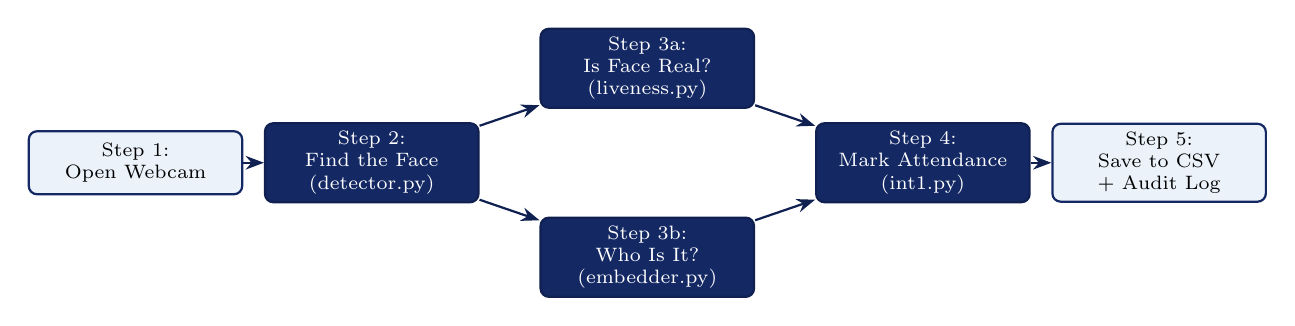
\begin{tikzpicture}[
  every node/.style={font=\scriptsize},
  mod/.style={rectangle, rounded corners=3pt, draw=SamsungBlue, fill=LightBg, text width=2.5cm, align=center, minimum height=0.8cm, inner sep=3pt},
  core/.style={rectangle, rounded corners=3pt, draw=SamsungBlue!80!black, fill=SamsungBlue, text=white, text width=2.5cm, align=center, minimum height=0.9cm, inner sep=3pt},
  every path/.style={>=Stealth, thick, draw=SamsungBlue!80!black}
]
\node[mod] (cam) at (-5.5, 0) {Step 1:\\Open Webcam};
\node[core] (det) at (-2.5, 0) {Step 2:\\Find the Face\\(detector.py)};
\node[core] (liv) at (1, 1.2) {Step 3a:\\Is Face Real?\\(liveness.py)};
\node[core] (emb) at (1, -1.2) {Step 3b:\\Who Is It?\\(embedder.py)};
\node[core] (app) at (4.5, 0) {Step 4:\\Mark Attendance\\(int1.py)};
\node[mod] (csv) at (7.5, 0) {Step 5:\\Save to CSV\\+ Audit Log};

\draw[->] (cam) -- (det);
\draw[->] (det) -- (liv);
\draw[->] (det) -- (emb);
\draw[->] (liv) -- (app);
\draw[->] (emb) -- (app);
\draw[->] (app) -- (csv);
\end{tikzpicture}
\end{center}
\end{frame}

% ===== SLIDE 7: SYSTEM ARCHITECTURE (Overview) =====
\begin{frame}{System Architecture --- Code Structure}
\begin{block}{Overview}
The system consists of 5 independent Python modules. The camera feeds frames to the detector, which then passes the aligned face to two modules running in parallel: one checks if the face is a living person, and the other identifies who it is. If both checks pass, attendance is recorded.
\end{block}
\vspace{10pt}
\begin{itemize}\setlength\itemsep{8pt}
  \item \textbf{Modular Design:} Each file handles exactly one job (detection, liveness, recognition, user interface, or anomaly detection). This makes the code clean and easy to upgrade.
  \item \textbf{Threaded Execution:} The entire recognition pipeline runs in a background thread. This ensures the main app window (Tkinter UI) stays smooth and responsive without freezing.
  \item \textbf{Lazy Initialization:} AI models are only loaded into memory when they are first needed, making the application start up much faster.
\end{itemize}
\end{frame}

% ===== SLIDE 7: ARCHITECTURE STEPS (Explanation) =====
\begin{frame}{System Architecture --- Step-by-Step Explanation}\small
\begin{block}{What happens from camera to attendance record?}\small
Here is what the system does every time someone stands in front of the camera:
\end{block}
\vspace{-2pt}
\footnotesize
\begin{enumerate}\setlength\itemsep{2pt}
  \item \textbf{Step 1 --- Open Webcam:} The camera starts recording at 30 fps. Old buffered frames are discarded.
  \item \textbf{Step 2 --- Find the Face:} The detector finds the face, marks 478 points on it, and straightens it into a 160$\times$160 image.
  \item \textbf{Step 3a --- Is the Face Real?} Liveness module runs CNN (MiniFASNet), movement analysis (MLVS), blood flow check (rPPG), and motion detection.
  \item \textbf{Step 3b --- Who Is It?} Recognition module converts the face into 512 numbers and compares with database using per-person thresholds (APBC).
  \item \textbf{Step 4 --- Mark Attendance:} If both checks pass, the app shows the name and asks for confirmation.
  \item \textbf{Step 5 --- Save Record:} Attendance saved to CSV file. Every event is written to an audit log.
\end{enumerate}
\end{frame}

% ===== SLIDE 8: DETECTION =====
\begin{frame}{How Face Detection Works (detector.py)}\small
\begin{columns}[T]
\column{0.52\textwidth}
\begin{block}{What happens when the camera sees a face?}
\small The system locates the face, marks key points, straightens it, and checks image quality.
\end{block}
\textbf{Step-by-step:}\\[2pt]
\footnotesize
\begin{enumerate}\setlength\itemsep{1pt}
  \item Camera captures a frame (one image from video).
  \item Brightness is improved using CLAHE enhancement.
  \item MediaPipe finds the face and places 478 dots on it.
  \item Five key points are used to straighten the face into a 160$\times$160 pixel image.
  \item A quality score is calculated based on sharpness, brightness, and head pose.
  \item Low-quality frames are skipped automatically.
\end{enumerate}
\column{0.46\textwidth}
\begin{block}{Quality Score}\scriptsize
A number between 0 and 1:\\[2pt]
\textbf{40\%} --- Sharpness (blur detection)\\[1pt]
\textbf{30\%} --- Brightness (not too dark/bright)\\[1pt]
\textbf{30\%} --- Head pose (facing camera)\\[2pt]
Below 0.30 $\to$ frame is discarded.
\end{block}
\begin{block}{Fixing Stale Frames}\scriptsize
Laptop cameras buffer old frames. We throw away 3 old frames before reading the latest one, so liveness checks always see the present.
\end{block}
\end{columns}
\end{frame}

% ===== SLIDE 9: NOVEL CONTRIBUTIONS =====
\begin{frame}{Summary of Novel Contributions}\small
\begin{block}{Four Custom Innovations for High Security}
\small We built four custom modules to make the system secure and adaptive, going beyond standard open-source attendance systems.
\end{block}
\vspace{4pt}
\begin{columns}[T]
\column{0.48\textwidth}
\textbf{1. MLVS (Micro-Landmark Velocity)}\\[2pt]
\footnotesize
Tracks tiny involuntary face movements (like breathing). Real faces show broad frequencies; photos and replays do not. Takes $<$3 ms to run.
\vspace{8pt}

\textbf{2. PACE (Progressive Challenge)}\\[2pt]
\footnotesize
If the AI is unsure if a face is real, it escalates the challenge. Asks the user to blink or turn their head, reducing false rejections for honest users.

\column{0.48\textwidth}
\textbf{3. APBC (Adaptive Calibration)}\\[2pt]
\footnotesize
Instead of one fixed matching score, each person gets a custom threshold based on their enrollment lighting, angles, and camera quality.
\vspace{8pt}

\textbf{4. TACE (Temporal Coherence)}\\[2pt]
\footnotesize
Checks attendance history to block proxies, replay attacks, and unusual time patterns (e.g., marking attendance at 3 AM).
\end{columns}
\end{frame}

% ===== SLIDE 13: DASHBOARD =====
\begin{frame}{Dashboard --- The User Interface}\small
\begin{block}{How does a user interact with the system?}
\small A desktop app built with Python's Tkinter. Simple buttons, no browser or internet needed.
\end{block}
\vspace{-2pt}
\begin{columns}[T]
\column{0.5\textwidth}
\textbf{App Features:}\\[2pt]
\footnotesize
\begin{itemize}\setlength\itemsep{1pt}
  \item \textbf{Enroll:} Admin enters password, types name, camera captures 10 samples with liveness check.
  \item \textbf{Mark Attendance:} Opens camera, checks liveness, recognizes face, saves record.
  \item \textbf{View / Export:} Table view of records. Excel export supported.
  \item \textbf{Manage Users:} List and delete enrolled people.
\end{itemize}
\column{0.48\textwidth}
\textbf{Security Features:}\\[2pt]
\footnotesize
\begin{itemize}\setlength\itemsep{1pt}
  \item \textbf{Admin password} for all sensitive actions.
  \item \textbf{Lockout:} 60-second lock after 3 failed attempts.
  \item \textbf{Duplicate block:} Same person cannot mark twice within 60 min.
  \item \textbf{Anti-clone:} Rejects if new face matches existing person ($>$72\%).
  \item \textbf{Voice feedback:} Speaks confirmation aloud.
  \item \textbf{Audit log:} Every event written to file.
\end{itemize}
\end{columns}
\end{frame}

% ===== SLIDE 12: SYSTEM WALKTHROUGH =====
\begin{frame}{System Walkthrough}
\begin{columns}[T]
\column{0.33\textwidth}
\begin{center}
\includegraphics[width=0.95\linewidth,height=3.5cm,keepaspectratio]{11.jpeg}
\vspace{4pt}\\
\textbf{1. UI}
\end{center}

\column{0.33\textwidth}
\begin{center}
\includegraphics[width=0.95\linewidth,height=3.5cm,keepaspectratio]{13.jpeg}
\vspace{4pt}\\
\textbf{2. Liveness Check}
\end{center}

\column{0.33\textwidth}
\begin{center}
\includegraphics[width=0.95\linewidth,height=3.5cm,keepaspectratio]{14.jpeg}
\vspace{4pt}\\
\textbf{3. Spoof detection}
\end{center}
\end{columns}
\end{frame}

% ===== SLIDE 16: RESULTS =====
\begin{frame}{Results and Analysis}\small
\begin{block}{How well does the system perform?}
\small We tested the system on a regular HP laptop with an Intel i5-1240P processor and a built-in 720p webcam. No GPU was used. Here are the results:
\end{block}
\vspace{-2pt}
\renewcommand{\arraystretch}{1.2}\footnotesize
\begin{tabular}{@{}p{3.8cm}p{1.8cm}p{7.5cm}@{}}
\toprule
\textbf{Metric} & \textbf{Result} & \textbf{Explanation}\\
\midrule
Recognition accuracy & $>$95\% & 19 out of 20 times, the correct person is identified.\\
Photo spoof rejection & 100\% & Printed photos are always caught and rejected.\\
Screen replay rejection & $>$95\% & Videos played on phone/laptop are almost always caught.\\
Time to enroll & $\sim$15 sec & 10 face samples captured at 0.7-second intervals.\\
Time to mark attendance & 2 to 8 sec & Depends on whether a blink challenge is needed (PACE zone).\\
AI model speed & $<$10 ms & The anti-spoofing model runs very fast per frame.\\
MLVS speed & $<$3 ms & The movement analysis is nearly instant.\\
\bottomrule
\end{tabular}
\end{frame}

% ===== SLIDE 17: CHALLENGES =====
\begin{frame}{Challenges and Solutions}
\renewcommand{\arraystretch}{1.25}\scriptsize
\begin{tabular}{@{}p{3cm}p{4.5cm}p{6cm}@{}}
\toprule
\textbf{Challenge We Faced} & \textbf{Why Did It Happen?} & \textbf{How We Fixed It}\\
\midrule
Wrong CNN scores on real faces & Fed a small cropped face image instead of a wider crop from the full frame. & Wrote a function to crop faces at exact zoom levels (2.7x, 4.0x) used during training.\\[2pt]
Camera showed old frames & Laptop cameras store old frames in memory, causing liveness checks to see the past. & Throw away 3 buffered frames before reading the latest one to ensure real-time analysis.\\[2pt]
Blink detection failed & Eye measurements used wrong units (tiny decimals instead of pixel distances). & Switched to pixel units and used relative thresholds (75\% of open-eye size = closed).\\[2pt]
MediaPipe API breakage & Google removed the old API in a newer version. & Rewrote the code to use the modern MediaPipe Tasks API.\\[2pt]
Photos accepted as real & A single AI model was not enough to catch all fakes. & Added MLVS (movement check) and optical flow on top of the CNN model.\\[2pt]
False rejections & Global threshold was too strict for dim lighting. & Built APBC to calculate a personalized threshold based on enrollment quality.\\
\bottomrule
\end{tabular}
\end{frame}

% ===== SLIDE 18: THANK YOU =====
\begin{frame}[plain]
\vspace*{1.8cm}
\begin{center}
{\Huge \textbf{Thank You!}}\\[12pt]
{\large Questions \& Discussion}\\[18pt]
\textbf{Shashi Kumar} --- 122AD0057\\[4pt]
Department of Artificial Intelligence and Data Science\\
Indian Institute of Information Technology,\\Design and Manufacturing, Kurnool\\[10pt]
%\includegraphics[width=0.12\textwidth]{iiitdm_logo.png}
\vspace{8pt}\\
{\small April 2026}
\end{center}
\end{frame}

\end{document}
